% Preambuła: definicja klasy dokumentu i lista potrzebnych pakietów ///////////////////////////////////////////////////////////////////////////////////////////////////////

\documentclass[12pt, a4paper]{report} % rozmiar czcionki, klasa dokumentu
\usepackage[left=2.5cm, right=2.5cm, top=3.5cm, bottom=3.5cm]{geometry} % ustawienia marginesów
\usepackage{amsmath} % przydatne przy pisaniu wzorów i symboli matematycznych
\usepackage{amssymb} % j.w.
\usepackage{amsthm} % j.w.
\usepackage{polski} % język polski i skład tekstu zgodnie z polskimi zasadami typografii
\usepackage[T1]{fontenc} % polskie fonty w formacie wektorowym
\usepackage[utf8]{inputenc} % j.w.
\usepackage{enumerate} % konfiguracja wyglądu wypunktowań (i) (ii) A) B) 1) 2) etc.
\usepackage[pdftex]{graphicx} % umieszczanie grafiki w pracy (w tym również w formacie wektorowym PDF)
\usepackage{indentfirst} % wcięcie pierwszego akapitu
\usepackage{booktabs} % do rysowania eleganckich tabel
\usepackage{color} % kolor w LaTeXu
\usepackage{pgfplots} % rysowanie wykresów i grafiki wektorowej
\pgfplotsset{compat=1.18}
\usepackage{titlesec} % zmiana wyglądu tytułów rozdziałów (czcionka, odległości między wierszami tytułów etc.)
\usepackage[position=t,justification=centering, singlelinecheck=off]{subfig} % pozwala umieszczać rysunki obok siebie; etykiety (a) (b) etc. nad rysunkiem i wycentrowane
\usepackage{fancyhdr} % formatowanie nagłówka, stopki i żywej paginy
\usepackage{microtype} % optymalne (wizualnie) odstępy między znakami - poprawia czytelność tekstu
\usepackage[pdftex]{hyperref} % tworzenie połączeń hipertekstowych (odnośników)
\usepackage{lmodern}
\usepackage{float}    % umożliwia [H] dla figur
\usepackage{caption}  % formatowanie podpisów
\usepackage{listings} % listingi kodu źródłowego
\usepackage{xcolor}   % kolory dla listingów

% Kolory i style listingów kodu
\definecolor{codegreen}{rgb}{0,0.6,0}
\definecolor{codegray}{rgb}{0.5,0.5,0.5}
\definecolor{codepurple}{rgb}{0.58,0,0.82}
\definecolor{backcolour}{rgb}{0.95,0.95,0.92}
\definecolor{codeblue}{rgb}{0,0,0.7}

\lstdefinestyle{cstyle}{
    backgroundcolor=\color{backcolour},
    commentstyle=\color{codegreen},
    keywordstyle=\color{codeblue}\bfseries,
    numberstyle=\tiny\color{codegray},
    stringstyle=\color{codepurple},
    basicstyle=\ttfamily\footnotesize,
    breaklines=true,
    captionpos=b,
    keepspaces=true,
    numbers=left,
    numbersep=5pt,
    showstringspaces=false,
    tabsize=2,
    language=C,
    frame=single,
    rulecolor=\color{codegray},
    literate={ą}{{\k{a}}}1 {ć}{{\'c}}1 {ę}{{\k{e}}}1 {ł}{{\l{}}}1
             {ń}{{\'n}}1 {ó}{{\'o}}1 {ś}{{\'s}}1 {ź}{{\'z}}1 {ż}{{\.z}}1
             {Ą}{{\k{A}}}1 {Ć}{{\'C}}1 {Ę}{{\k{E}}}1 {Ł}{{\L{}}}1
             {Ń}{{\'N}}1 {Ó}{{\'O}}1 {Ś}{{\'S}}1 {Ź}{{\'Z}}1 {Ż}{{\.Z}}1
}

\lstdefinestyle{pythonstyle}{
    backgroundcolor=\color{backcolour},
    commentstyle=\color{codegreen},
    keywordstyle=\color{codeblue}\bfseries,
    numberstyle=\tiny\color{codegray},
    stringstyle=\color{codepurple},
    basicstyle=\ttfamily\footnotesize,
    breaklines=true,
    captionpos=b,
    keepspaces=true,
    numbers=left,
    numbersep=5pt,
    showstringspaces=false,
    tabsize=2,
    language=Python,
    frame=single,
    rulecolor=\color{codegray},
    literate={ą}{{\k{a}}}1 {ć}{{\'c}}1 {ę}{{\k{e}}}1 {ł}{{\l{}}}1
             {ń}{{\'n}}1 {ó}{{\'o}}1 {ś}{{\'s}}1 {ź}{{\'z}}1 {ż}{{\.z}}1
             {Ą}{{\k{A}}}1 {Ć}{{\'C}}1 {Ę}{{\k{E}}}1 {Ł}{{\L{}}}1
             {Ń}{{\'N}}1 {Ó}{{\'O}}1 {Ś}{{\'S}}1 {Ź}{{\'Z}}1 {Ż}{{\.Z}}1
}

% Konfiguracja nagłówka, stopki (w tym wyglądu i sposobu numeracji stron) i wyglądu tytułów głównych rozdziałów ///////////////////////////////////////////////

\pagestyle{fancy}
\cfoot{\thepage}
\fancyhead{} % czyści wszystkie pola w nagłówku
\fancyhead[RO,LE]{\textit {\textsl{Projekt i budowa układu regulacji dla układu Ball on Beam} \ldots}} % tekst w nagłówku
\fancyfoot{} % czyści wszystkie pola w stopce
\fancyfoot[C]{\thepage} % numery stron w stopce; wycentrowane

\titleformat{\chapter}[display]
  {\normalfont\Large\raggedleft}
  {\MakeUppercase{\chaptertitlename}
    \rlap{ \resizebox{!}{1.5cm}{\thechapter} \rule{5cm}{1.5cm}}}
  {10pt}{\Huge}
\titlespacing*{\chapter}{0pt}{30pt}{50pt} % odstępy w tytule głównym



% Początek dokumenty ///////////////////////////////////////////////////////////////////////////////////////////////////////////////////////////////////////////////////////////////
\begin{document}

  % Strona tytułowa
\begin{titlepage}

\vspace*{-2cm} % odstęp pionowy

\begin{center} % wypośrodkuj
\Large \textbf{POLITECHNIKA POZNAŃSKA}\\[1mm]
\Large {WYDZIAŁ AUTOMATYKI, ROBOTYKI I ELEKTROTECHNIKI}\\[1mm]
\begin{large}
Instytut Robotyki i Inteligencji Maszynowej\\[1mm]
Zakład Automatyki i Optymalizacji\\[1cm]
\end{large}
\end{center}

\begin{center}

\includegraphics[height=3cm,keepaspectratio]{img/logo.pdf}
\end{center}

\vspace{1cm}

\begin{center}
\Large \textbf {Jan Andrzejewski \\ Mateusz Banaszak \\ Piotr Bednarek}
\end{center}

\vspace{1cm}

\begin{center}
\Large \textbf{\textit{PROJEKT I BUDOWA UKŁADU REGULACJI DLA UKŁADU BALL ON BEAM}}
\end{center}

\vspace{3cm}
\hfill
\textbf {Promotor}: dr inż. Jacek Michalski

\vspace{2cm}

 \hspace*{-1cm}
\begin{minipage}{7cm}
\centering
Pracę przyjmuję i akceptuję\\

\vspace{0.5cm}

................................................\\

\textit{\footnotesize data i podpis opiekuna pracy}
\end{minipage}

\vspace{2.5cm}

\begin{center}
Poznań, \the\year
\end{center}


  % Pusta strona  (w tym miejscu karta tematu z Dziekanatu) \\\\\\\\\\\\\\\\\\\\\\\\\\\\\\\\\\\\\\\\\\\\\\\\\\\\\\\\\\\\\\\\\\\\\\\\\\\\\\\\\\\\\\\\\\\\\\\\\\\\\\\\\\\\\\\\\\
\newpage\null\thispagestyle{empty}\newpage


 % Streszczenie \\\\\\\\\\\\\\\\\\\\\\\\\\\\\\\\\\\\\\\\\\\\\\\\\\\\\\\\\\\\\\\\\\\\\\\\\\\\\\\\\\\\\\\\\\\\\\\\\\\\\\\\\\\\\\\\\\\\\\\\\\\\\\\\\\\\\\\\\\\\\\\\\\\\\\\\\\\\\\\\\\\\\\\
    \newpage\thispagestyle{empty}
    \vspace*{2\baselineskip}
    \begin{center}
	{\large\bfseries Streszczenie}\par\bigskip
    \end{center}

    {\itshape
    Praca przedstawia projekt i~budowę autonomicznego stanowiska do sterowania
    pozycją kulki na belce (\textit{ball and beam}) z~wykorzystaniem mikrokontrolera
    STM32F767ZI.
    Opisano budowę mechaniczną stanowiska, zastosowane peryferia (serwomechanek
    MG946R, czujnik odległości VL53L0X, rząd diod LED, potencjometr) oraz
    architekturę oprogramowania opartą na systemie FreeRTOS.
    Wyprowadzono model matematyczny układu i~zaprojektowano dwa regulatory:
    klasyczny PID z~anti-windup oraz optymalny LQR w~przestrzeni stanów.
    Aplikacja nadzorcza napisana w~Pythonie (PySide6) umożliwia wizualizację
    sygnałów w~czasie rzeczywistym, zapis danych do pliku CSV oraz zdalne
    strojenie regulatora.
    Przeprowadzono weryfikację eksperymentalną i~potwierdzono spełnienie
    wszystkich wymagań projektowych.
    }
    \vspace*{1\baselineskip}

    \noindent{\bf Słowa kluczowe}: {\itshape regulacja automatyczna, kulka na belce,
    STM32, PID, LQR, FreeRTOS, VL53L0X.}
    \par
    \vspace{4\baselineskip}

  % Abstract \\\\\\\\\\\\\\\\\\\\\\\\\\\\\\\\\\\\\\\\\\\\\\\\\\\\\\\\\\\\\\\\\\\\\\\\\\\\\\\\\\\\\\\\\\\\\\\\\\\\\\\\\\\\\\\\\\\\\\\\\\\\\\\\\\\\\\\\\\\\\\\\\\\\\\\\\\\\\\\\\\\\\\\\\\\
    \begin{center}
	{\large\bfseries Abstract}\par\bigskip
    \end{center}
    \noindent{\bf Title}: {\itshape Design and Construction of a Control System for the Ball and Beam System.}\par
    \vspace*{1\baselineskip}
    {\itshape
    This thesis presents the design and construction of an autonomous ball-and-beam
    control system based on the STM32F767ZI microcontroller.
    The mechanical setup, hardware peripherals (MG946R servo, VL53L0X time-of-flight
    sensor, LED bar, potentiometer), and FreeRTOS-based software architecture are
    described.
    A mathematical model of the plant is derived and two controllers are designed:
    a classical PID with anti-windup and an optimal LQR state-feedback controller.
    A supervisory desktop application (Python/PySide6) provides real-time signal
    visualisation, CSV data logging, and remote parameter tuning.
    Experimental verification confirms that all project requirements are satisfied.
    }
    \vspace*{1\baselineskip}

    \noindent{\bf Key words}: {\itshape automatic control, ball and beam, STM32, PID,
    LQR, FreeRTOS, VL53L0X.}

\end{titlepage}

  % Spis treści ]\\\\\\\\\\\\\\\\\\\\\\\\\\\\\\\\\\\\\\\\\\\\\\\\\\\\\\\\\\\\\\\\\\\\\\\\\\\\\\\\\\\\\\\\\\\\\\\\\\\\\\\\\\\\\\\\\\\\\\\\\\\\\\\\\\\\\\\\\\\\\\\\\\\\\\\\\\\\\\\\\\\\\\\\\

\tableofcontents % wstawia spis treści

 % Główna część pracy \\\\\\\\\\\\\\\\\\\\\\\\\\\\\\\\\\\\\\\\\\\\\\\\\\\\\\\\\\\\\\\\\\\\\\\\\\\\\\\\\\\\\\\\\\\\\\\\\\\\\\\\\\\\\\\\\\\\\\\\\\\\\\\\\\\\\\\\\\\\\\\\\\\


% ROZDZIAŁ 1 _________________________________________________________________________________________________________________
% ROZDZIAŁ 1: Wprowadzenie

\chapter{Wprowadzenie}

\section{Cel i zakres pracy}

\section{Przegląd literatury}

\section{Struktura pracy}


% ROZDZIAŁ 2 _________________________________________________________________________________________________________________
% ROZDZIAŁ 2: Budowa stanowiska i oprogramowanie

\chapter{Budowa stanowiska i oprogramowanie}
\label{ch:budowa}

Niniejszy rozdział opisuje fizyczną budowę stanowiska laboratoryjnego, zastosowane
komponenty elektroniczne, środowisko programistyczne oraz architekturę oprogramowania
sterującego — firmware mikrokontrolera i~aplikację nadzorczą.

% -----------------------------------------------------------------------
\section{Opis stanowiska laboratoryjnego}
% -----------------------------------------------------------------------

Stanowisko składa się z~wydrukowanej w~technologii 3D pochyłej belki, po której
swobodnie toczy się metalowy walec (kulka).
Kąt nachylenia belki kontrolowany jest przez serwomechanek połączony z~belką
za pomocą dźwigni.
Pozycja kulki mierzona jest bezdotykowo za pomocą czujnika odległości ToF
zamontowanego na końcu belki.
Mikrokontroler STM32 odczytuje pomiar z~czujnika, oblicza sygnał sterujący
i~generuje odpowiedni sygnał PWM dla serwa.

\begin{figure}[H]
  \centering
  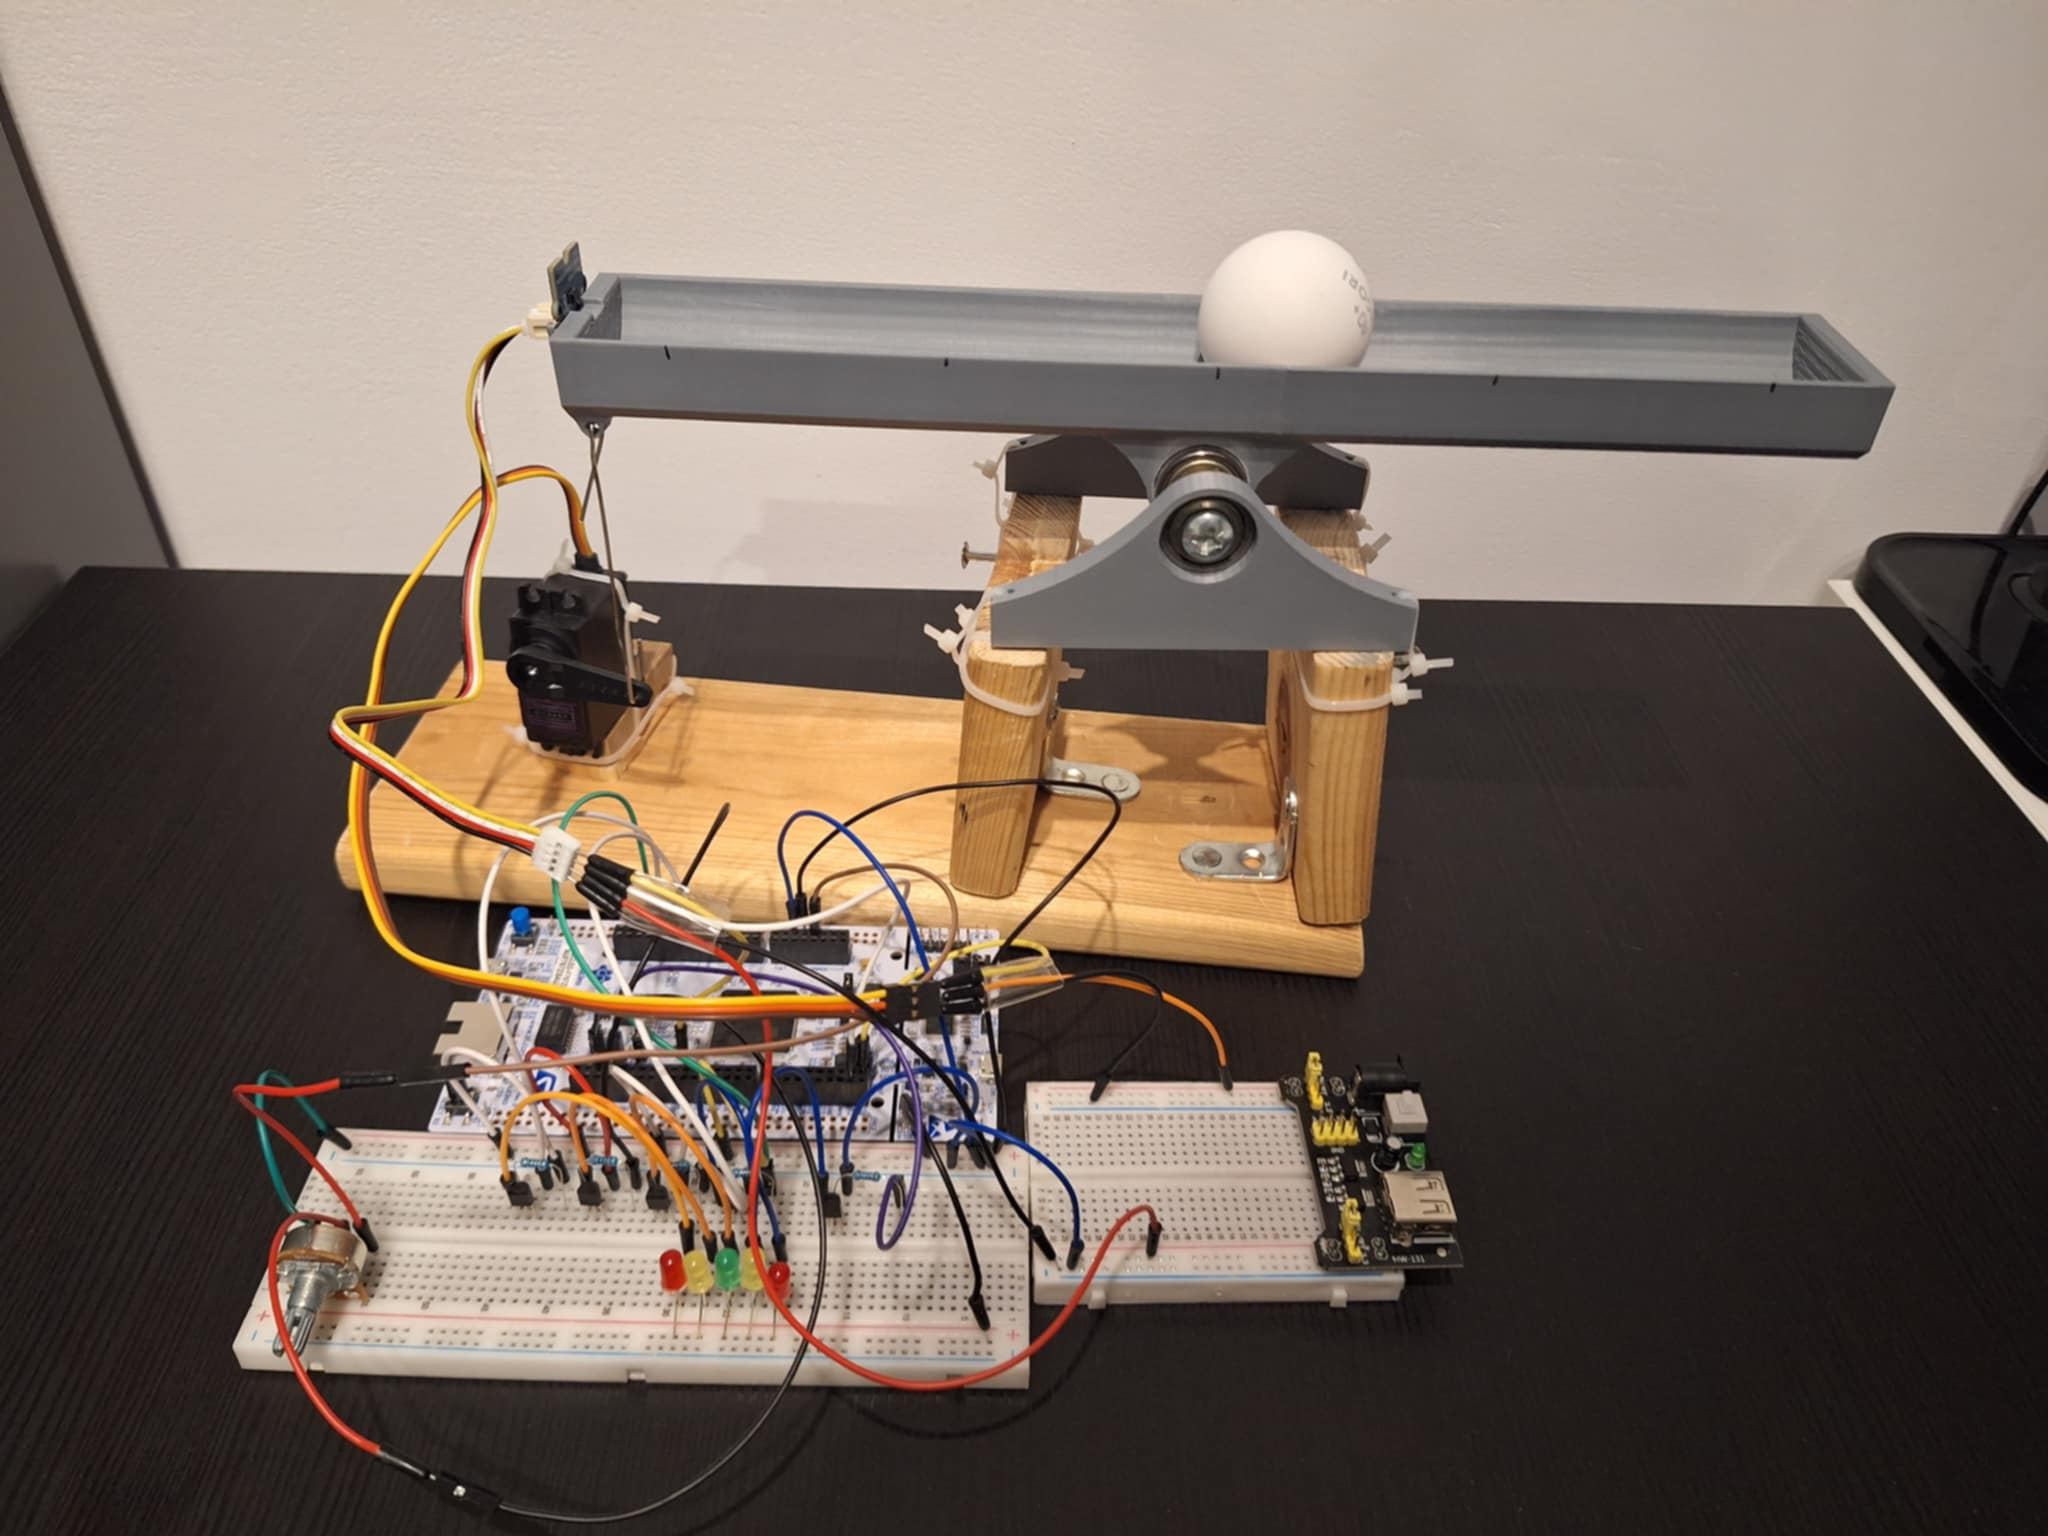
\includegraphics[width=0.8\linewidth]{2-budowa-stanowiska-i-oprogramowanie/2-img/stanowisko.png}
  \caption{Stanowisko laboratoryjne układu kulka na belce}
  \label{fig:stanowisko}
\end{figure}

\subsection{Wykaz komponentów}

\begin{table}[H]
  \centering
  \caption{Komponenty sprzętowe stanowiska}
  \label{tab:komponenty}
  \begin{tabular}{lll}
    \toprule
    \textbf{Element} & \textbf{Model / opis} & \textbf{Interfejs} \\
    \midrule
    Mikrokontroler & STM32 Nucleo F767ZI & --- \\
    Serwomechanek  & TowerPro MG946R      & PWM 50\,Hz \\
    Czujnik odległości & Grove VL53L0X ToF & I\textsuperscript{2}C \\
    Potencjometr   & liniowy & ADC (PA0) \\
    Zasilacz       & 5\,V DC & --- \\
    \bottomrule
  \end{tabular}
\end{table}

% -----------------------------------------------------------------------
\section{Mikrokontroler STM32 i peryferia}
% -----------------------------------------------------------------------

\subsection{Mikrokontroler STM32F767ZI}

Głównym procesorem stanowiska jest mikrokontroler STM32F767ZI~\cite{stm32f767zi}
zamontowany na płytce ewaluacyjnej Nucleo-F767ZI.
Układ oparty jest na rdzeniu ARM Cortex-M7 taktowanym z~częstotliwością 216\,MHz
i~wyposażony jest w~bogatą gamę peryferiów: kilka interfejsów I\textsuperscript{2}C
i UART, timery sprzętowe, przetwornik ADC oraz obsługę sygnałów PWM.

\begin{figure}[H]
  \centering
  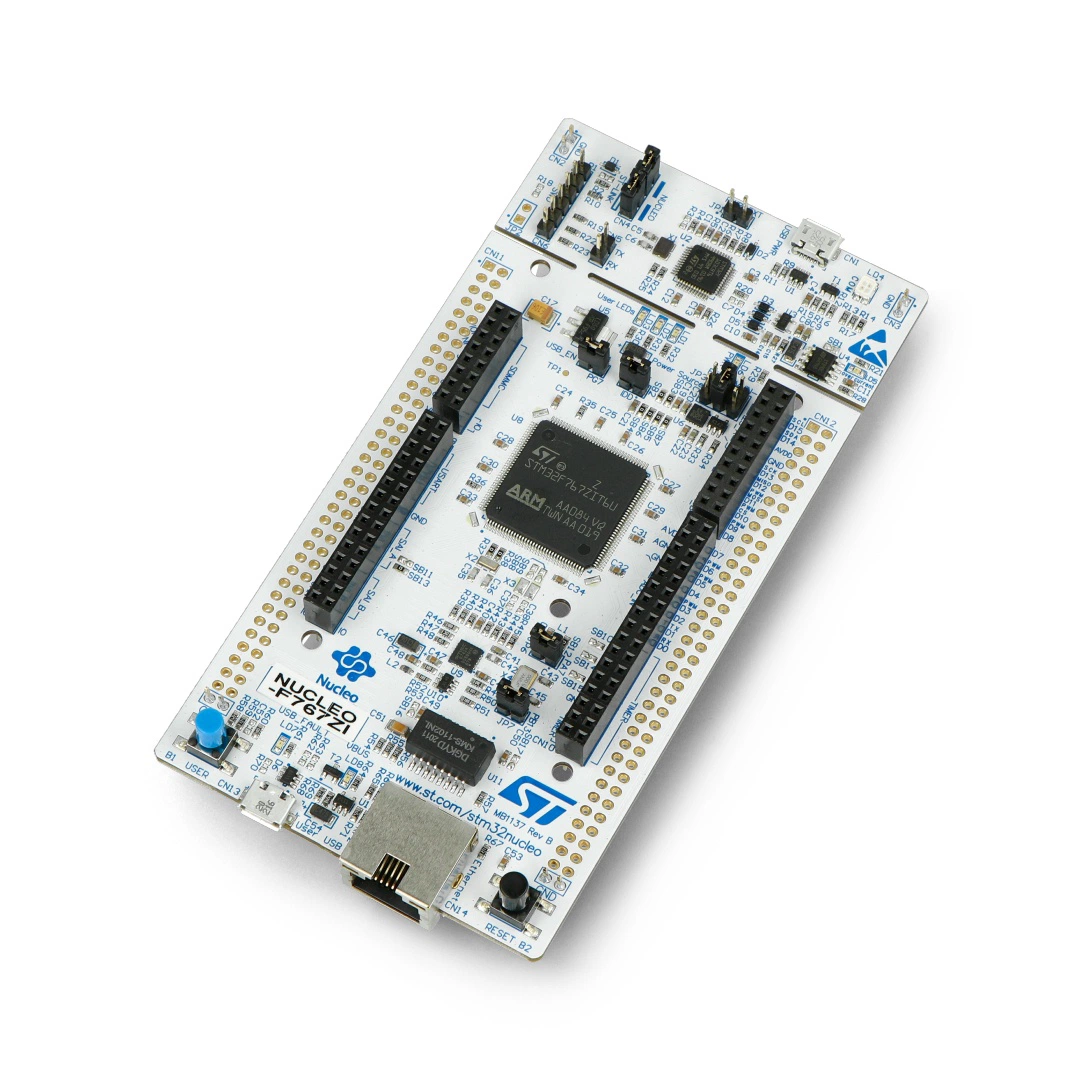
\includegraphics[width=0.45\linewidth]{2-budowa-stanowiska-i-oprogramowanie/2-img/plytka.png}
  \caption{Płytka ewaluacyjna STM32 Nucleo-F767ZI}
\end{figure}

\subsection{Serwomechanek MG946R}

Do sterowania kątem belki zastosowano serwomechanek TowerPro MG946R.
Serwo przyjmuje sygnał PWM o~częstotliwości 50\,Hz i~czasie wypełnienia
od 1\,ms (pełne wychylenie w~jedną stronę) do 2\,ms (pełne wychylenie
w~drugą stronę).
Zakres roboczy ograniczony jest w~oprogramowaniu do 60--140° w~celu
zabezpieczenia mechaniki.

\begin{figure}[H]
  \centering
  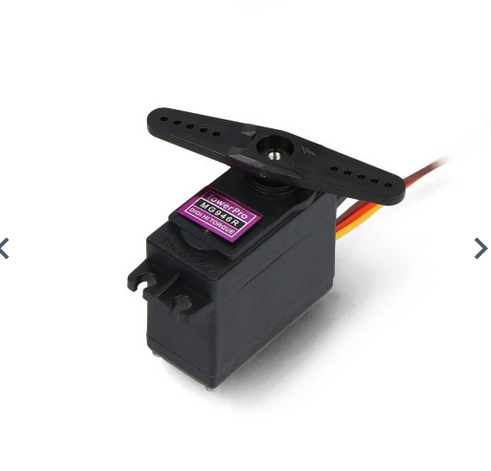
\includegraphics[width=0.35\linewidth]{2-budowa-stanowiska-i-oprogramowanie/2-img/servo.png}
  \caption{Serwomechanek TowerPro MG946R}
\end{figure}

\subsection{Czujnik odległości VL53L0X}

Pozycja kulki mierzona jest czujnikiem VL53L0X~\cite{vl53l0x} firmy
STMicroelectronics, pracującym w~technologii Time-of-Flight (ToF).
Czujnik emituje krótkie impulsy laserowe podczerwieni i~mierzy czas
powrotu odbitego sygnału, co pozwala wyznaczyć odległość z~rozdzielczością
1\,mm w~zakresie do 2\,m.
Komunikacja z~mikrokontrolerem odbywa się przez magistralę I\textsuperscript{2}C.

\begin{figure}[H]
  \centering
  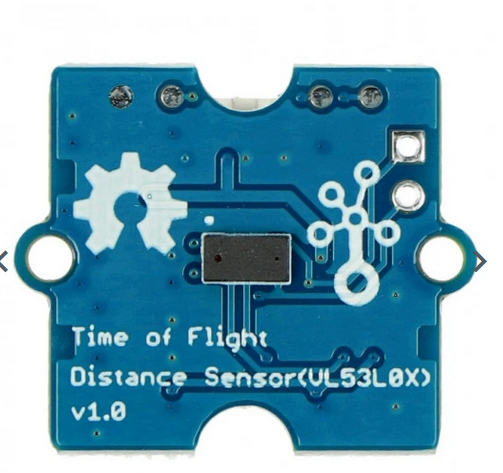
\includegraphics[width=0.4\linewidth]{2-budowa-stanowiska-i-oprogramowanie/2-img/sensor.png}
  \caption{Czujnik odległości Grove VL53L0X Time-of-Flight}
\end{figure}

\subsection{Potencjometr}

Potencjometr liniowy podłączony do wejścia analogowego PA0 (ADC1\_CH0)
umożliwia ręczne zadawanie wartości referencyjnej pozycji kulki
w~trybie analogowym.
Przetwornik ADC skonfigurowany jest z~rozdzielczością 12-bitową
($0$--$4095$), co odpowiada zakresowi pozycji $0$--$250\,\mathrm{mm}$.

% -----------------------------------------------------------------------
\section{Środowisko programistyczne}
% -----------------------------------------------------------------------

\subsection{Firmware STM32}

Oprogramowanie mikrokontrolera zostało opracowane w~środowisku
STM32CubeIDE (Eclipse CDT ze zintegrowanym kompilatorem ARM GCC).
Konfigurację peryferiów (timery, I\textsuperscript{2}C, UART, ADC, PWM)
wygenerowano za pomocą narzędzia STM32CubeMX.
Kod źródłowy podzielono na osobne moduły~C zgodnie ze standardem Doxygen:

\begin{table}[H]
  \centering
  \caption{Moduły firmware}
  \label{tab:moduly}
  \begin{tabular}{ll}
    \toprule
    \textbf{Moduł} & \textbf{Opis} \\
    \midrule
    \texttt{main.c/h}       & Główna aplikacja, konfiguracja peryferiów \\
    \texttt{servo\_pid.c/h} & Regulator PID z~anti-windup \\
    \texttt{lqr.c/h}        & Regulator LQR (przestrzeń stanów) \\
    \texttt{filters.c/h}    & Filtry cyfrowe (EMA, mediana, 1-Euro) \\
    \texttt{crc8.c/h}       & Suma kontrolna CRC-8 \\
    \texttt{calibration.c/h}& Kalibracja czujnika VL53L0X \\
    \texttt{vl53l0x.c/h}    & Sterownik czujnika (I\textsuperscript{2}C) \\
    \bottomrule
  \end{tabular}
\end{table}

System operacyjny czasu rzeczywistego FreeRTOS zarządza wykonaniem dwóch
wątków (tasków):
\begin{itemize}
  \item \texttt{ControlTask} (priorytet wysoki) — pętla sterowania;
  \item \texttt{DefaultTask} (priorytet normalny) — obsługa komend UART.
\end{itemize}

\subsection{Aplikacja desktopowa}

Aplikacja nadzorcza napisana jest w~języku Python~3 z~wykorzystaniem
frameworka PySide6 (Qt~6).
Zapewnia ona:
\begin{itemize}
  \item połączenie z~mikrokontrolerem przez port szeregowy (pyserial),
  \item wizualizację sygnałów w~czasie rzeczywistym (pyqtgraph),
  \item zadawanie wartości referencyjnej i~nastaw regulatorów,
  \item nagrywanie danych i~eksport do pliku CSV,
  \item podgląd kamery z~detekcją pozycji kulki (OpenCV).
\end{itemize}

\begin{figure}[H]
  \centering
  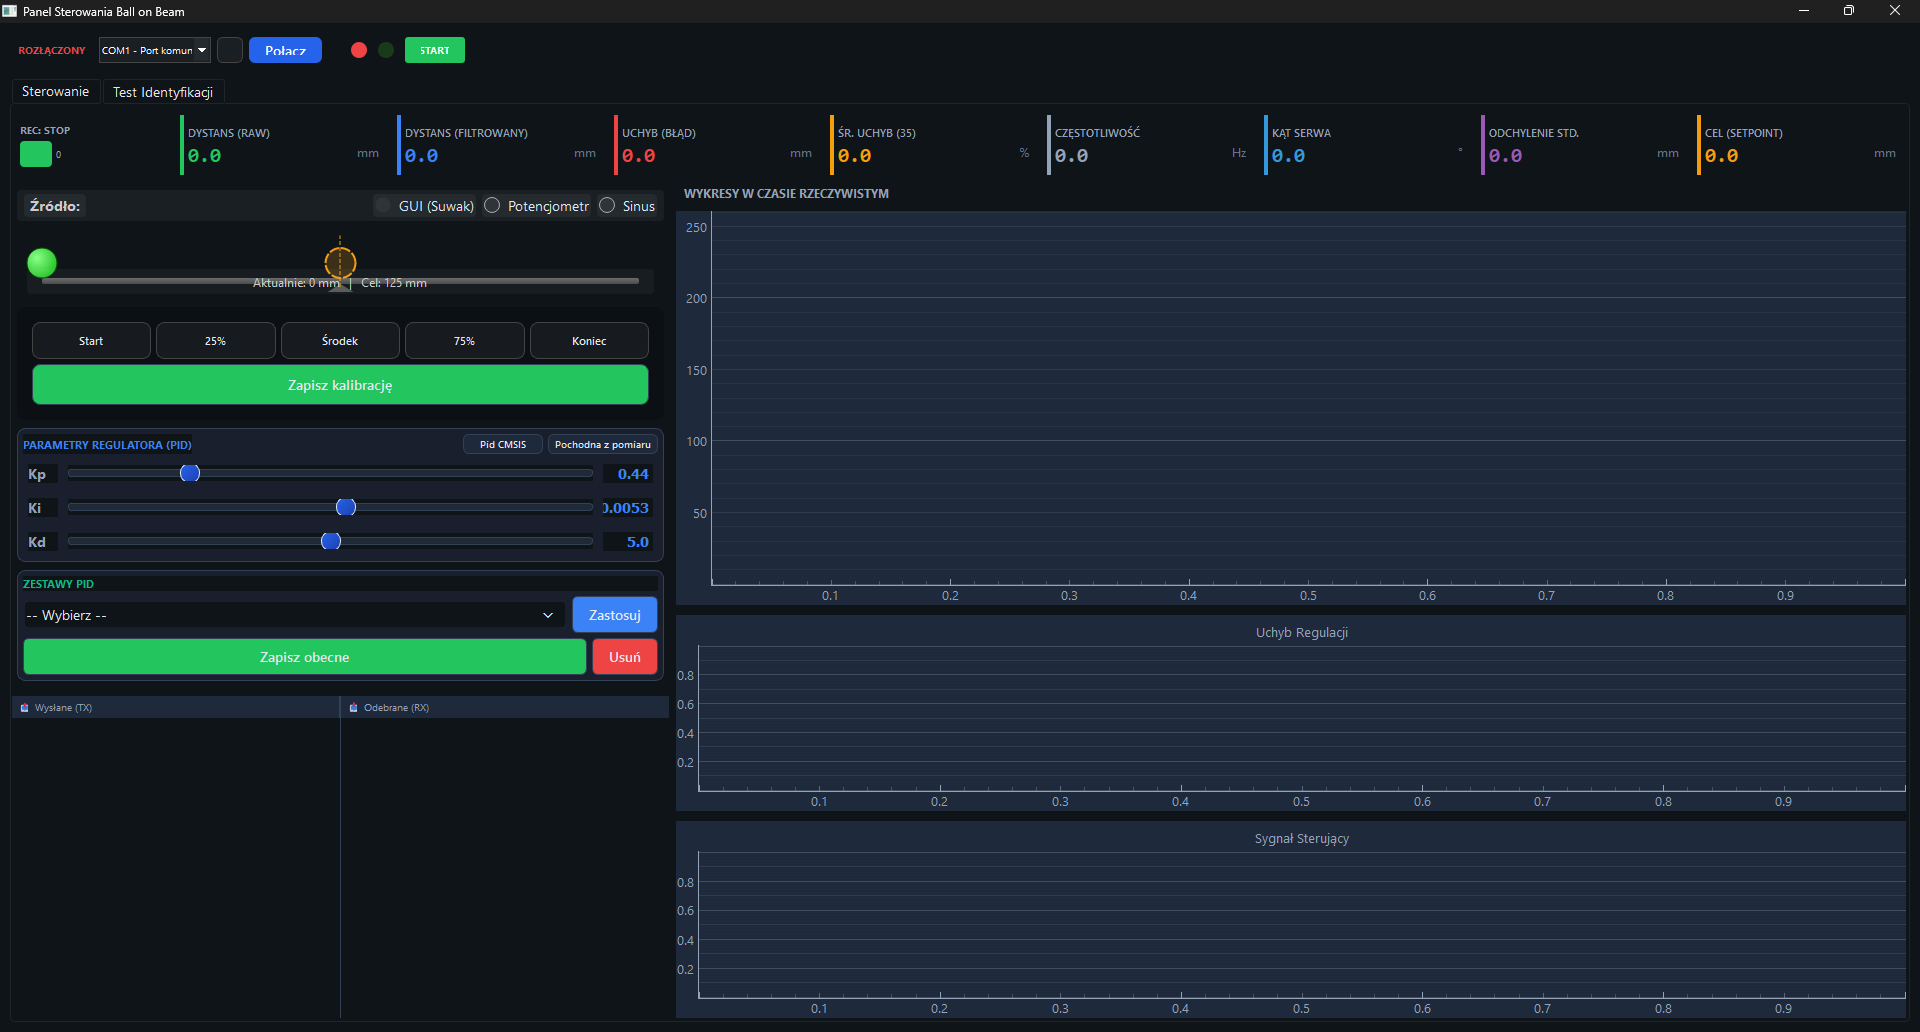
\includegraphics[width=0.9\linewidth]{2-budowa-stanowiska-i-oprogramowanie/2-img/desktop.png}
  \caption{Okno aplikacji desktopowej (PySide6)}
  \label{fig:desktop}
\end{figure}

% -----------------------------------------------------------------------
\section{Implementacja algorytmu sterowania}
% -----------------------------------------------------------------------

\subsection{Pętla sterowania i okres próbkowania}

Algorytm sterowania realizowany jest przez \texttt{ControlTask} z~ustalonym
okresem próbkowania 30\,ms wymuszonym przez funkcję \texttt{osDelay()}:

\begin{lstlisting}[style=cstyle, caption={Stały okres próbkowania w pętli sterowania (main.c)}]
#define PID_DT_MS 30

for (;;) {
    distance = readRangeContinuousMillimeters(&distanceStr);

    // obliczenia regulatora ...

    SetServoAngle(pid_output);
    osDelay(PID_DT_MS); // staly okres 30 ms
}
\end{lstlisting}

\subsection{Ograniczenie zakresu serwa}

Wyjście regulatora jest nasycane do bezpiecznego zakresu kąta serwa:

\begin{lstlisting}[style=cstyle, caption={Saturacja wyjścia i ograniczenia serwa (main.c)}]
#define SERVO_MIN_LIMIT  60.0f
#define SERVO_MAX_LIMIT 140.0f

if (pid_angle < SERVO_MIN_LIMIT)  pid_angle = SERVO_MIN_LIMIT;
if (pid_angle > SERVO_MAX_LIMIT)  pid_angle = SERVO_MAX_LIMIT;
SetServoAngle(pid_angle);
\end{lstlisting}

\subsection{Protokół telemetrii UART z sumą kontrolną CRC-8}

Dane pomiarowe przesyłane są przez UART~3 (115200\,baud) w~formacie
tekstowym z~sumą kontrolną CRC-8 (wielomian 0x07).
Format ramki:
\[
\texttt{D:\%d;Z:\%d;A:\%d;F:\%d;E:\%d;V:\%d;S:\%d;C:\%02X\textbackslash r\textbackslash n}
\]
gdzie kolejne pola oznaczają: surowy dystans, setpoint, kąt serwa,
dystans filtrowany, uchyb, średni uchyb, status czujnika i~CRC.

\begin{lstlisting}[style=cstyle, caption={Implementacja CRC-8 (crc8.c)}]
uint8_t CalculateCRC8(const char *data, int len) {
    uint8_t crc = 0x00;
    for (int i = 0; i < len; i++) {
        crc ^= data[i];
        for (uint8_t j = 0; j < 8; j++) {
            if (crc & 0x80)
                crc = (crc << 1) ^ 0x07;
            else
                crc <<= 1;
        }
    }
    return crc;
}
\end{lstlisting}

\subsection{Zadania FreeRTOS}

System operacyjny czasu rzeczywistego tworzy dwa wątki:

\begin{lstlisting}[style=cstyle, caption={Tworzenie zadań FreeRTOS (main.c)}]
osThreadDef(defaultTask, StartDefaultTask,
            osPriorityNormal, 0, 256);
defaultTaskHandle = osThreadCreate(osThread(defaultTask), NULL);

osThreadDef(ControlTask, StartControlTask,
            osPriorityHigh, 0, 1024);
ControlTaskHandle = osThreadCreate(osThread(ControlTask), NULL);

osKernelStart();
\end{lstlisting}



% ROZDZIAŁ 3 _________________________________________________________________________________________________________________
% ROZDZIAŁ 3: Model matematyczny i projekt regulacji

\chapter{Model matematyczny i projekt regulacji}
\label{ch:model}

\section{Model matematyczny obiektu regulacji}

\section{Identyfikacja parametrów modelu}

\section{Projekt regulatora}

\section{Symulacja układu regulacji}


% ROZDZIAŁ 4 _________________________________________________________________________________________________________________
% ROZDZIAŁ 4: Wyniki eksperymentalne

\chapter{Wyniki eksperymentalne}

\section{Metodyka przeprowadzonych badań}

\section{Wyniki pomiarów}

\section{Analiza i omówienie wyników}


% ROZDZIAŁ 5 _________________________________________________________________________________________________________________
% ROZDZIAŁ 5: Podsumowanie i wnioski

\chapter{Podsumowanie i wnioski}

\section{Podsumowanie}

\section{Wnioski}

\section{Kierunki dalszych badań}



% BIBLIOGRAFIA ___________________________________________________________________________________________________________
\bibliographystyle{unsrt} % kolejność cytowania w tekście
\bibliography{bibliografia}

\listoffigures
\appendix

\end{document}
